
\section{Výsledná aplikace}

\begin{figure}[H]
    \centering
    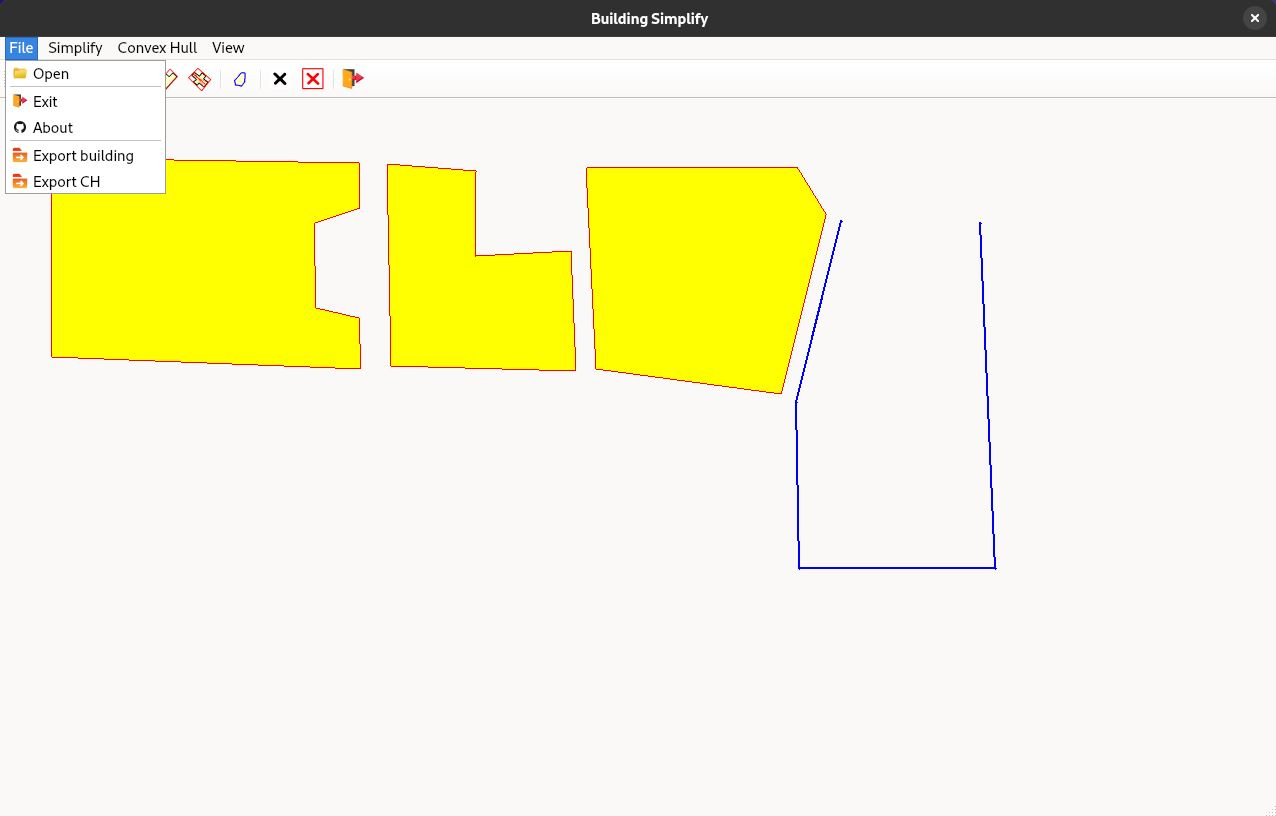
\includegraphics[width=\textwidth]{images/Ukazaka_aplikace.JPG}
    \caption{Ukázka vzhledu výsledné aplikace}
\end{figure}

\begin{figure}[H]
    \centering
    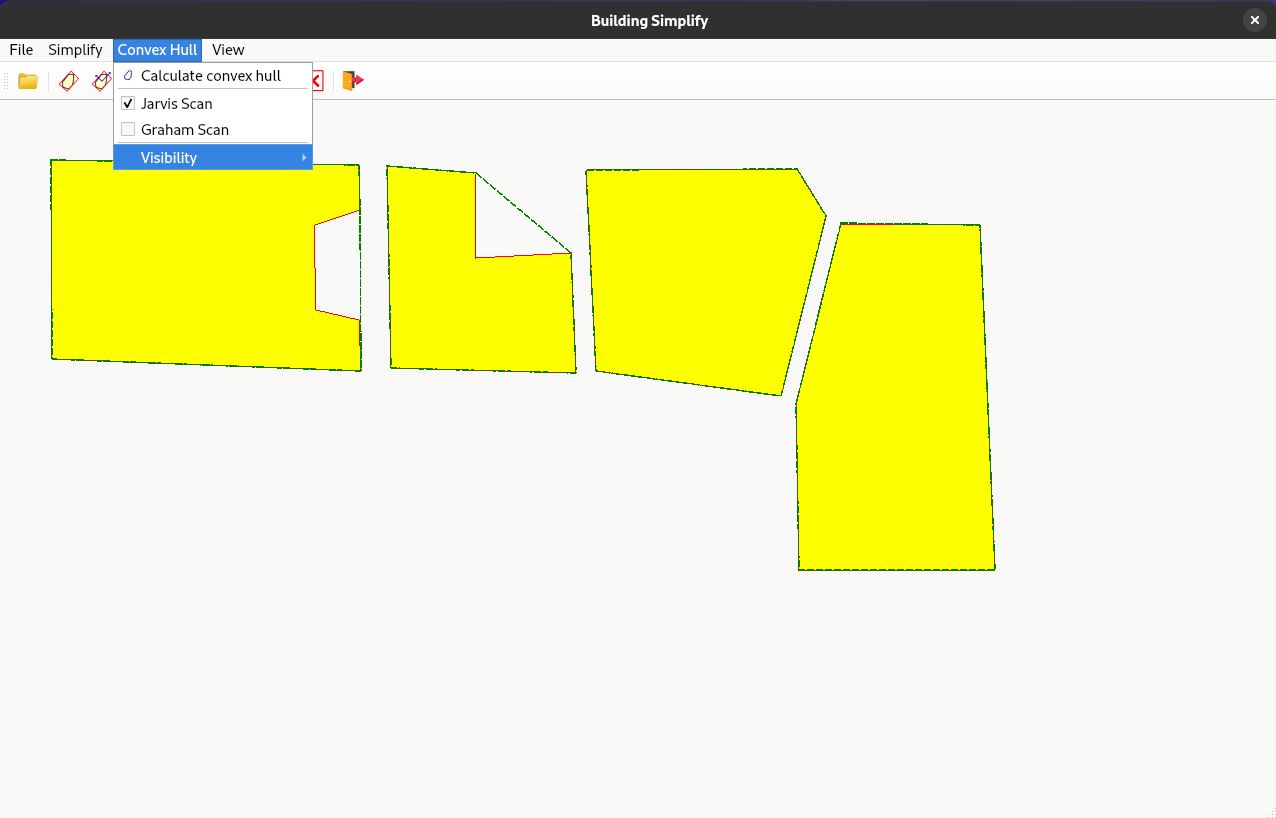
\includegraphics[width=\textwidth]{images/Ukazaka_ch.JPG}
    \caption{Tvorba konvexní obálky}
\end{figure}

\begin{figure}[H]
    \centering
    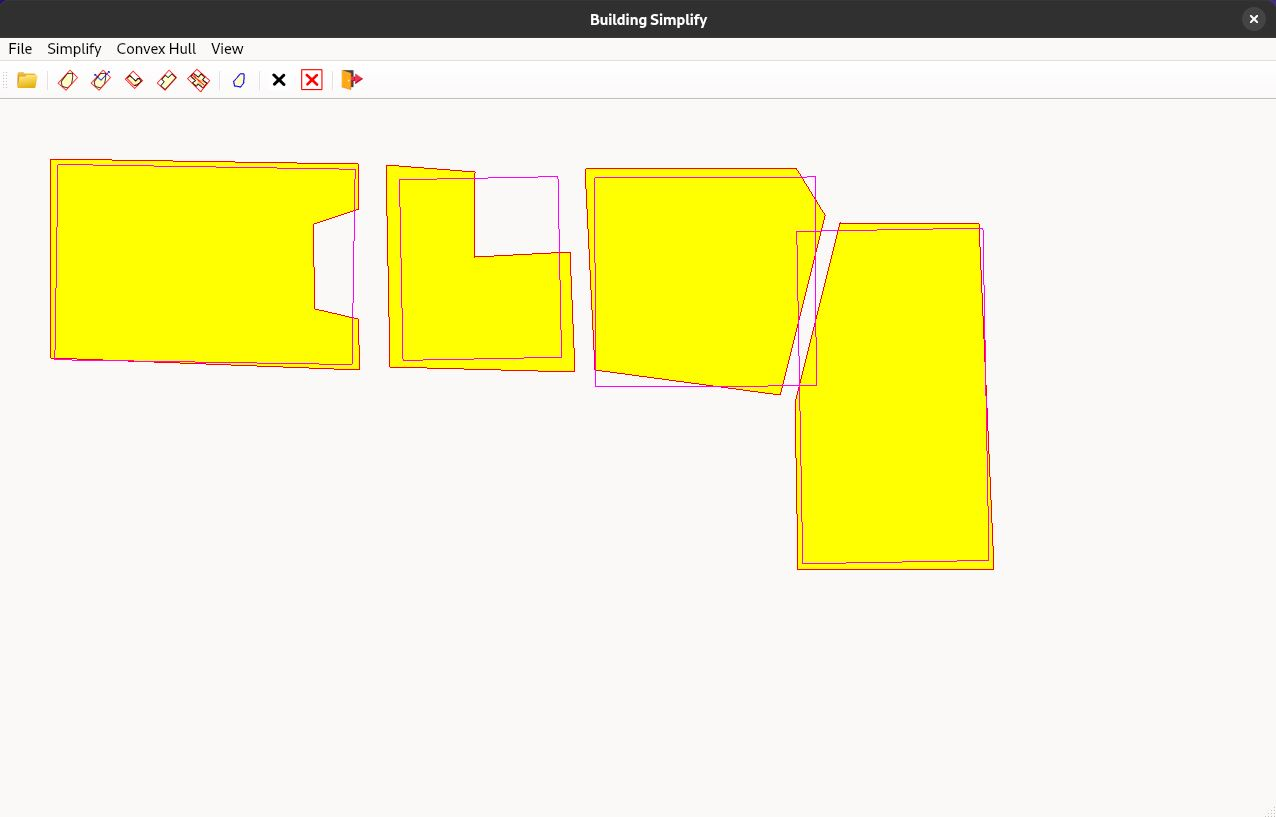
\includegraphics[width=\textwidth]{images/Ukazaka_maer.JPG}
    \caption{Generalizace metodou Minimum Area Enclosing Rectangle}
\end{figure}

\begin{figure}[H]
    \centering
    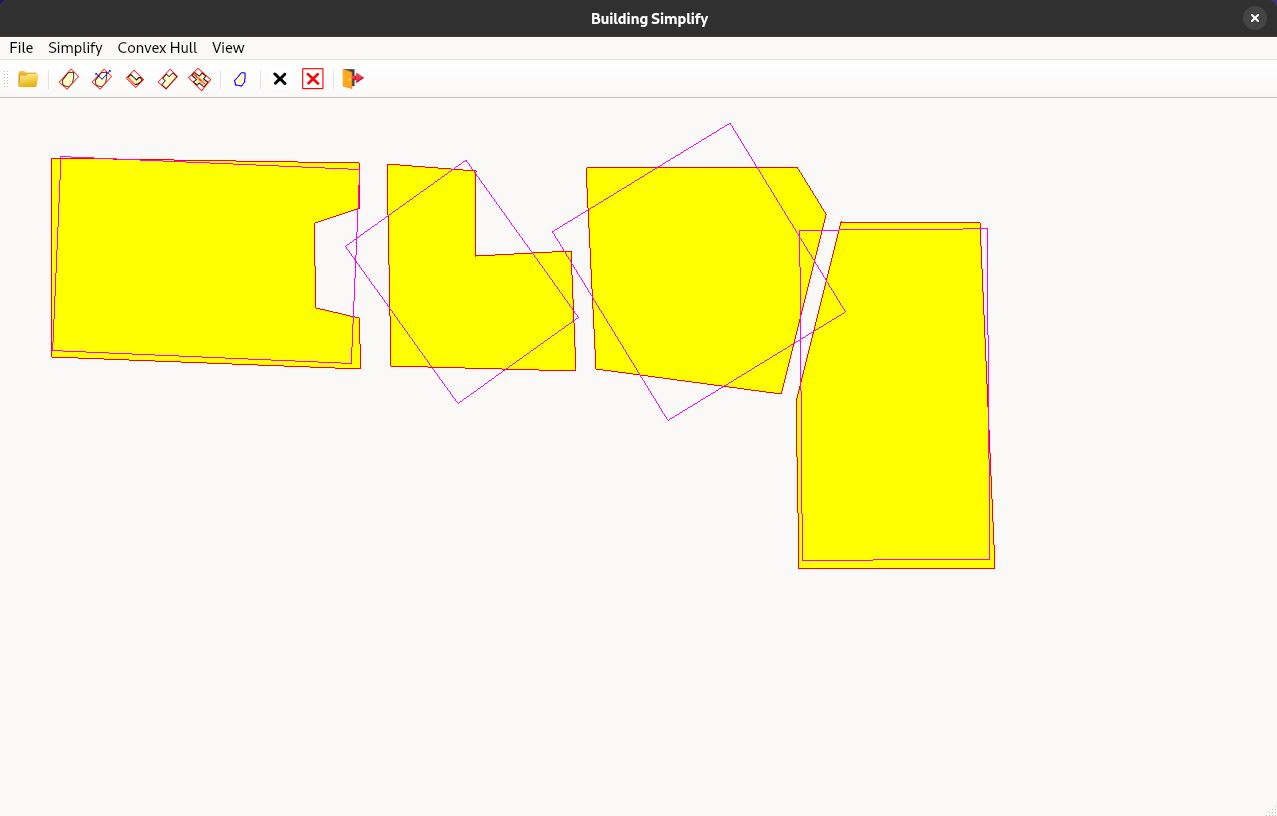
\includegraphics[width=\textwidth]{images/Ukazaka_pca.JPG}
    \caption{Generalizace metodou PCA}
\end{figure}

\begin{figure}[H]
    \centering
    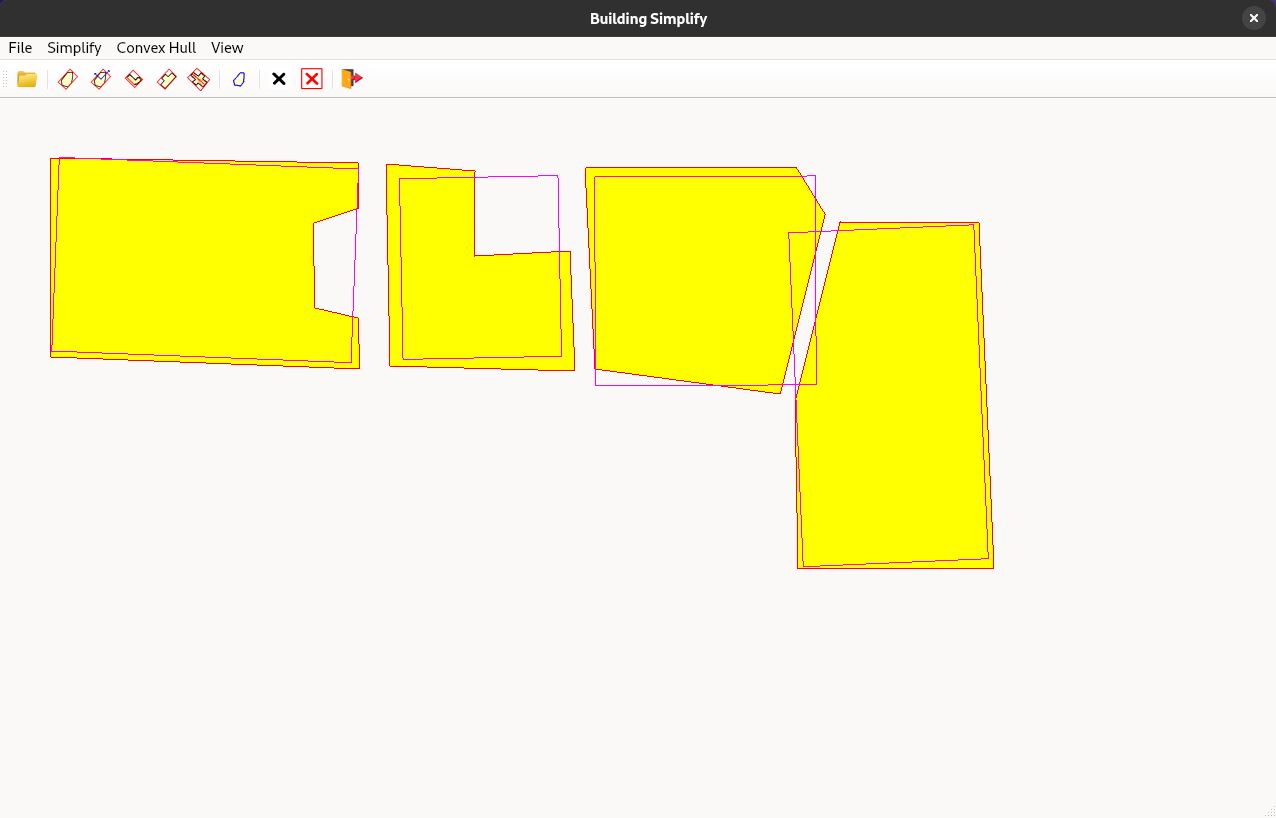
\includegraphics[width=\textwidth]{images/Ukazaka_le.JPG}
    \caption{Generalizace metodou Longest Edge}
\end{figure}

\begin{figure}[H]
    \centering
    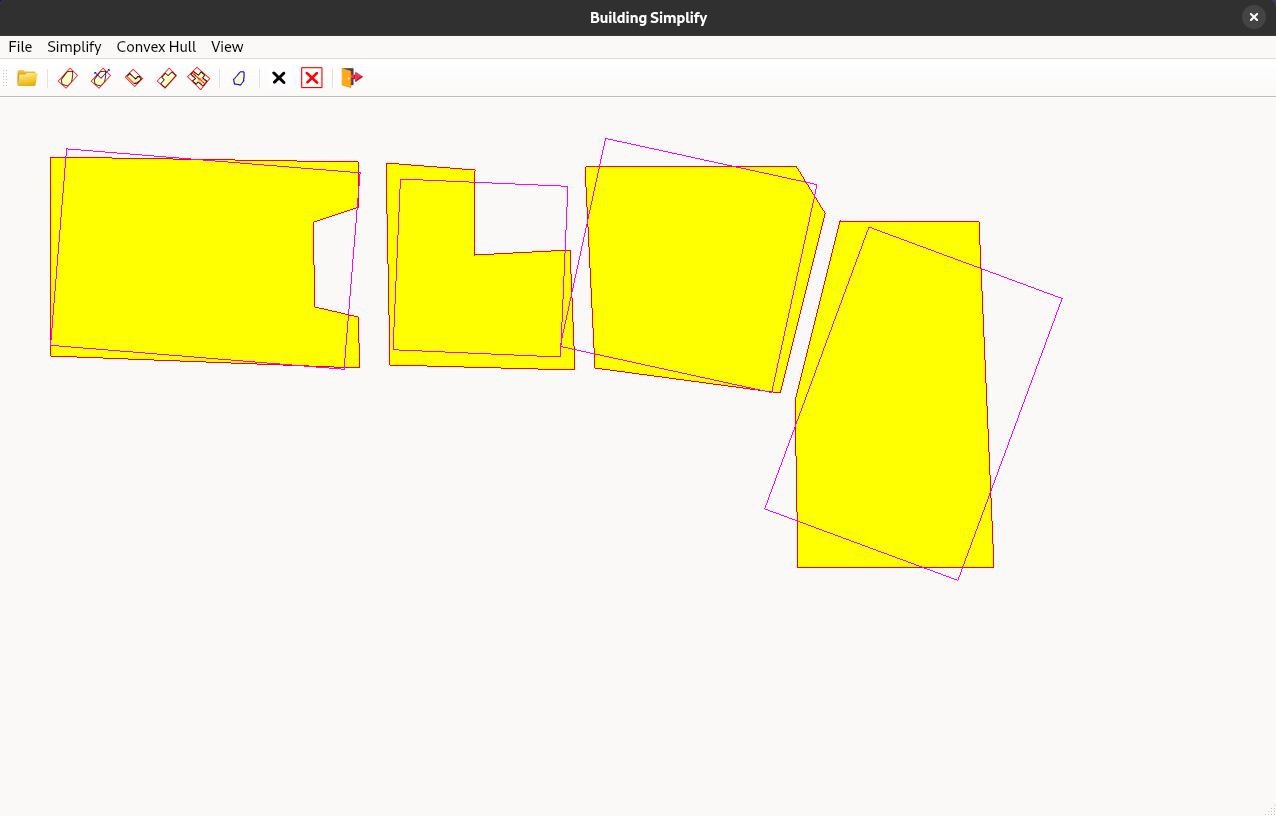
\includegraphics[width=\textwidth]{images/Ukazaka_wa.JPG}
    \caption{Generalizace metodou Wall Average}
\end{figure}

\begin{figure}[H]
    \centering
    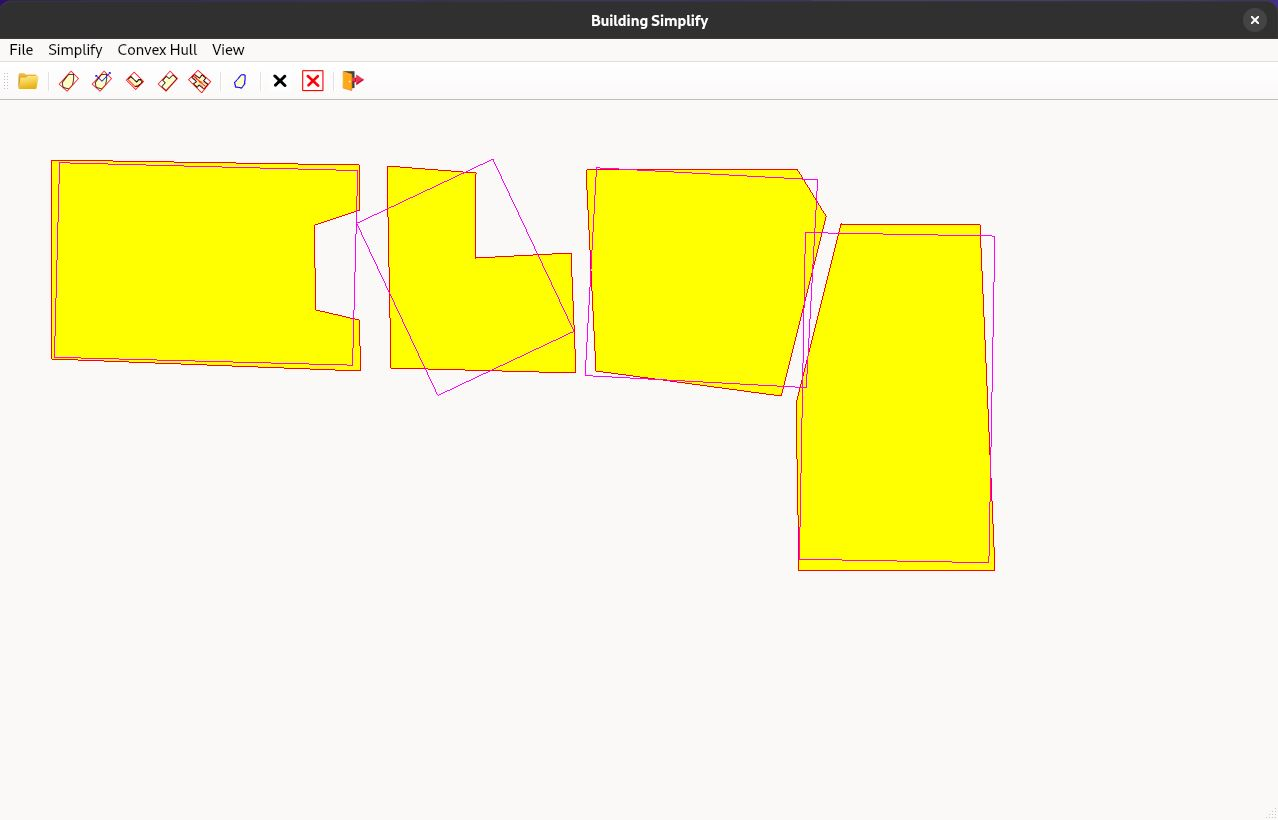
\includegraphics[width=\textwidth]{images/Ukazaka_wb.JPG}
    \caption{Generalizace metodou Weighted Bisector}
\end{figure}

\begin{figure}[H]
    \centering
    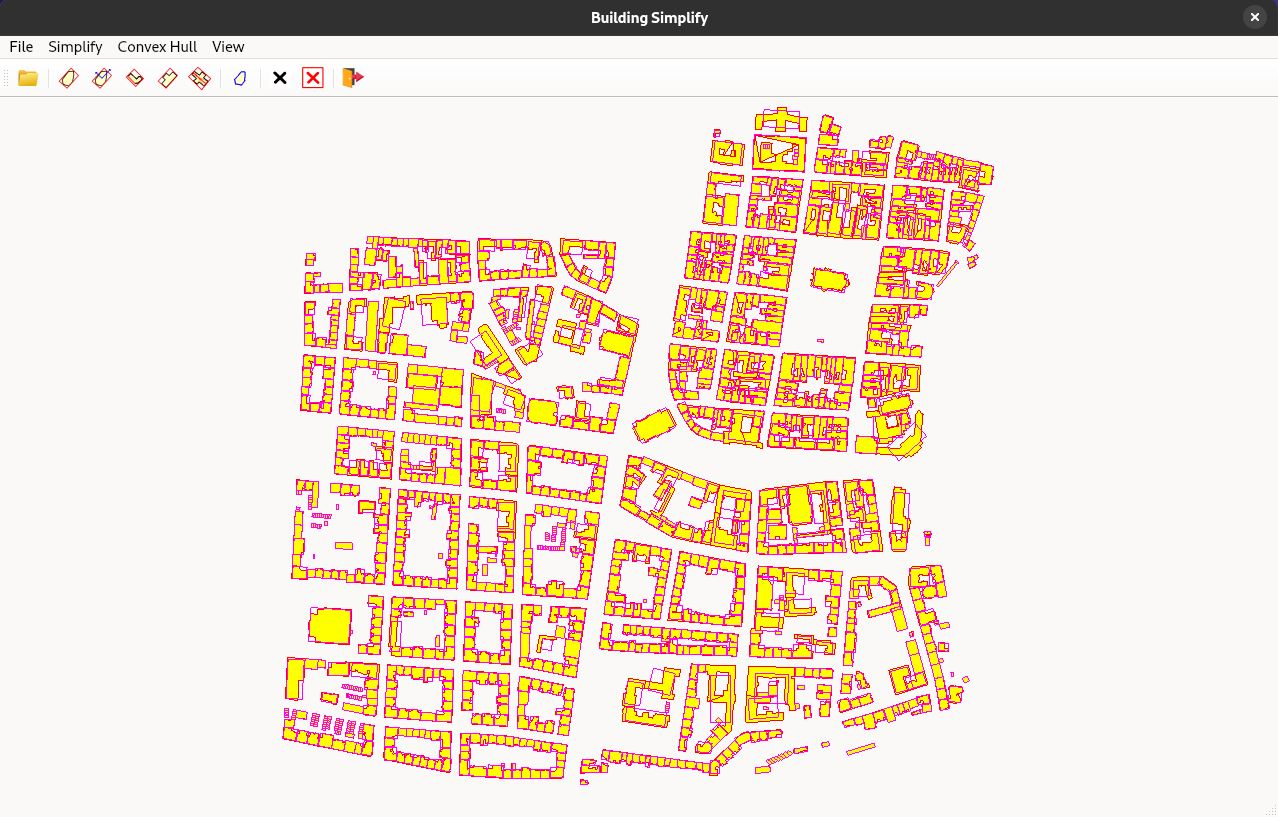
\includegraphics[width=\textwidth]{images/Ukazaka_city_centre.JPG}
    \caption{Generalizace budov v centru města metodou MAER}
\end{figure}


\begin{figure}[H]
    \centering
    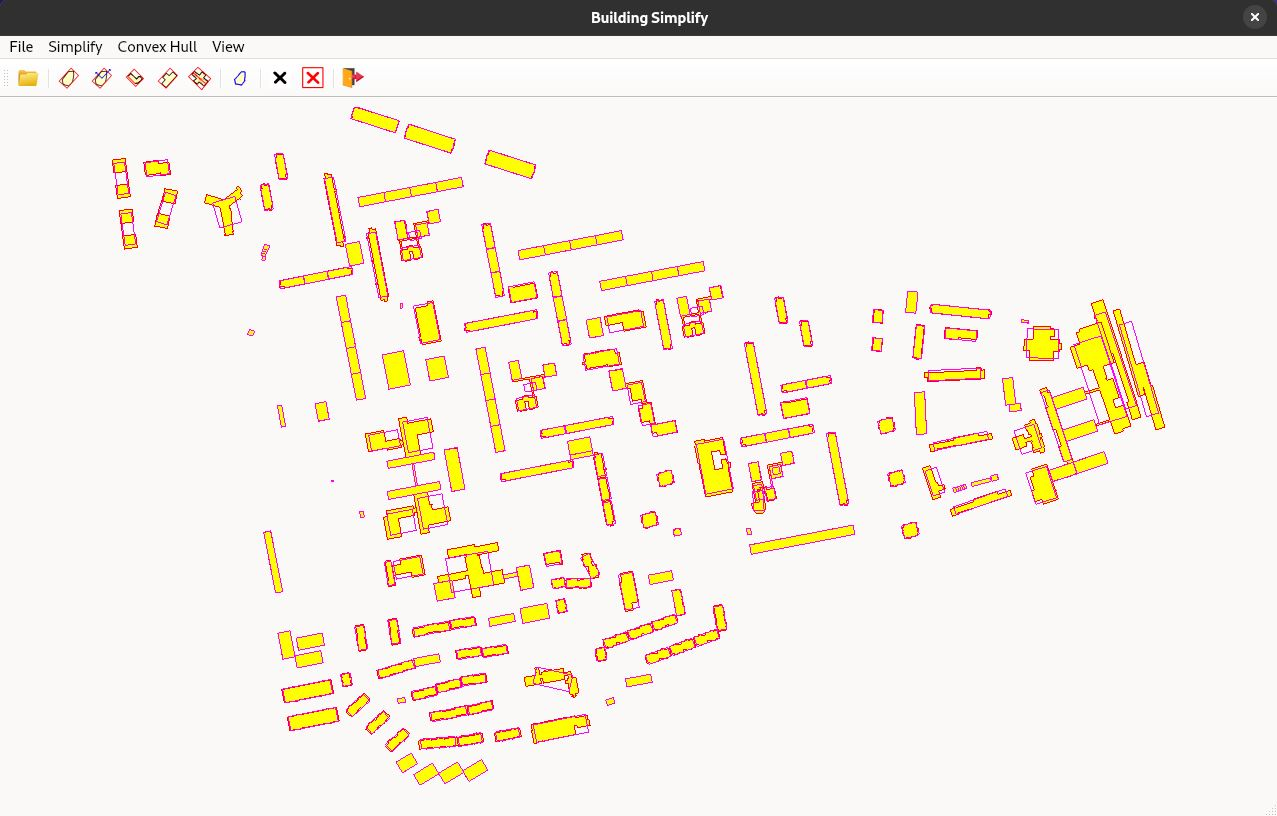
\includegraphics[width=\textwidth]{images/Ukazaka_block.JPG}
    \caption{Generalizace budov panelového sídliště metodou MAER}
\end{figure}

\begin{figure}[H]
    \centering
    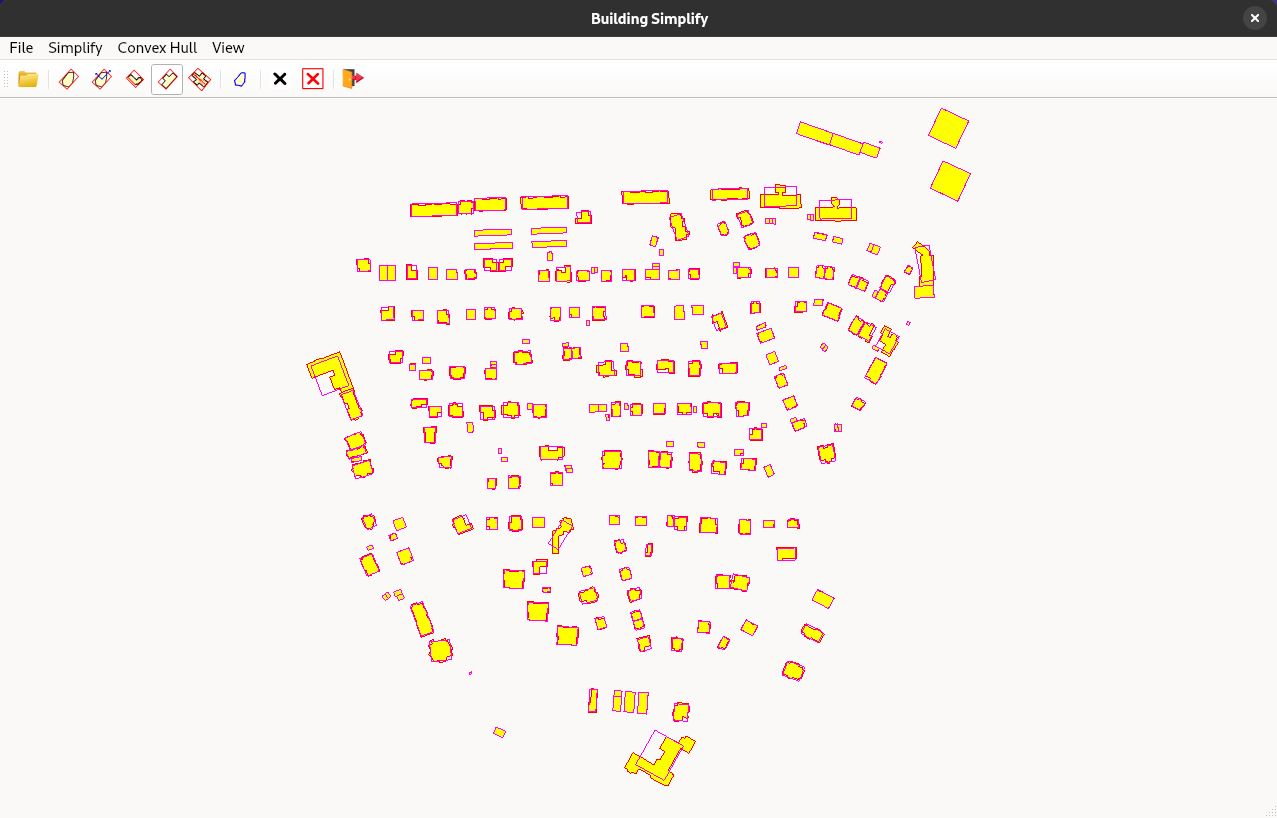
\includegraphics[width=\textwidth]{images/Ukazaka_villa_district.JPG}
    \caption{Generalizace budov ve vilové čtvrti metodou MAER}
\end{figure}